

%----------------------------------------------------------------------------------------
%	PACKAGES AND OTHER DOCUMENT CONFIGURATIONS 
%----------------------------------------------------------------------------------------

\documentclass[paper=a4, fontsize=11pt]{scrartcl} % A4 paper and 11pt font size



\usepackage[T1]{fontenc} % Use 8-bit encoding that has 256 glyphs
\usepackage{fourier} % Use the Adobe Utopia font for the document - comment this line to return to the LaTeX default
\usepackage[english]{babel} % English language/hyphenation
\usepackage{amsmath,amsfonts,amsthm} % Math packages

\usepackage{lipsum} % Used for inserting dummy 'Lorem ipsum' text into the template

\usepackage{sectsty} % Allows customizing section commands
\allsectionsfont{\centering \normalfont\scshape} % Make all sections centered, the default font and small caps

\usepackage{graphicx}

\usepackage{fancyhdr} % Custom headers and footers
\pagestyle{fancyplain} % Makes all pages in the document conform to the custom headers and footers
\fancyhead{} % No page header - if you want one, create it in the same way as the footers below
\fancyfoot[L]{} % Empty left footer
\fancyfoot[C]{} % Empty center footer
%\fancyfoot[R]{\thepage} % Page numbering for right footer
\renewcommand{\headrulewidth}{0pt} % Remove header underlines
\renewcommand{\footrulewidth}{0pt} % Remove footer underlines
\setlength{\headheight}{13.6pt} % Customize the height of the header

\numberwithin{equation}{section} % Number equations within sections (i.e. 1.1, 1.2, 2.1, 2.2 instead of 1, 2, 3, 4)
\numberwithin{figure}{section} % Number figures within sections (i.e. 1.1, 1.2, 2.1, 2.2 instead of 1, 2, 3, 4)
\numberwithin{table}{section} % Number tables within sections (i.e. 1.1, 1.2, 2.1, 2.2 instead of 1, 2, 3, 4)

\setlength\parindent{0pt} % Removes all indentation from paragraphs - comment this line for an assignment with lots of text

%----------------------------------------------------------------------------------------
%	TITLE SECTION
%----------------------------------------------------------------------------------------

\newcommand{\horrule}[1]{\rule{\linewidth}{#1}} % Create horizontal rule command with 1 argument of height

\title{	
\normalfont \normalsize 
\textsc{School of Electrical \& Information Engineering, University of the
Witwatersrand, Private Bag 3, 2050, Johannesburg, South Africa} \\ [25pt] % Your university, school and/or department name(s)
\horrule{0.5pt} \\[0.4cm] % Thin top horizontal rule
\huge Sprint Backlog \\ % The assignment title
\horrule{2pt} \\[0.5cm] % Thick bottom horizontal rule
}

\author{} % Your name

\date{\normalsize\today} % Today's date or a custom date

\begin{document}

\maketitle % Print the title

%----------------------------------------------------------------------------------------
%	PROBLEM 1
%----------------------------------------------------------------------------------------


%----------------------------------------------------------------------------------------
\newpage
\section{SCRUM}

The agile software development framework chosen for the project was the SCRUM method. This method was chosen because it is lightweight, simple to understand and easy to use. Scrum will be used to address complex problems, increase productivity and deliver a unique solution. An iterative process will be followed where one team is responsible for the front-end and the other team is responsible for the back-end. The process will be iterative whereby the front end team will develop the web pages and the back-end team will then link these pages to the server. It will also be assumed that product specifications will remain constant for the prototype phase with any changes been added after the development of the prototype

\subsection{The project chart}
The various components of the project chart is described in the introduction of this document.
\subsection{Product Backlog}
The product backlog can be seen in Table 1.1 
\begin{table}[!hbt]
\centering
\caption{product Backlog}
\label{my-label}
\begin{tabular}{|p{1cm}|p{8cm}|p{2cm}|p{1.2cm}|}
\hline
\textbf{ID} & \textbf{Story}                                                                                         & \textbf{Estimate} & \textbf{Priority} \\ \hline
1           & As a sender I need to be able to create an account                                                     & 10                & 1                 \\ \hline
2           & As a sender I need to be able to log in to my account                                                  & 2                 & 2                 \\ \hline
3           & As a sender I need to input the dimensions of my package                                               & 2                 & 3                 \\ \hline
4           & As a sender I want to input my details                                                                 & 3                 & 4                 \\ \hline
5           & As a sender I want to input the receiver's details                                                     & 2                 & 5                 \\ \hline
6           & As a sender I need to be able to pay for the services                                                  & 5                 & 6                 \\ \hline
7           & As a fleet assigment manager I need to be able run a route generation algorithm                        & 5                 & 7                 \\ \hline
8           & As a fleet assigment manager I need to see a list of packages in the depot                             & 1                 & 8                 \\ \hline
9           & As a driver I should be able to log in to my account                                                   & 1                 & 9                 \\ \hline
10          & As a driver I want to pick a vehicle and a route                                                       & 10                & 10                \\ \hline
11          & As a driver I need to see the contact details of my next delivery / pickup                             & 2                 & 11                \\ \hline
12          & As a driver I want to check off the packages I drop off / pickup                                       & 3                 & 12                \\ \hline
13          & As a sender I need to know when the parcel will be picked up                                           & 1                 & 13                \\ \hline
14          & As a sender I need to be able to know when the package will be delivered                               & 3                 & 14                \\ \hline
15          & As a receiver I need to receive a notification of the intended delivery                                & 1.5               & 15                \\ \hline
16          & As a receiver I need to check the estimated time of delivery                                           & 1                 & 16                \\ \hline
17          & As the CEO I want to see statistics on the clients                                                     & 4                 & 17                \\ \hline
18          & As the CEO I want to see statistics on the drivers                                                     & 4                 & 18                \\ \hline
19          & As the Vehicle Maintenance Manager I want to see vehicle statistics such as mileage                    & 6                 & 19                \\ \hline
20          & As the Vehicle Maintenance Manager I want to schedule the maintenance of vehicles                      & 5                 & 20                \\ \hline
21          & As the Accounts Officer I want to see the list of payments made (for bookeeping purposes)              & 6                 & 21                \\ \hline
22          & As the Accounts Officer I need to see a list of vehicle maintenance payments (for bookeeping purposes) & 5                 & 22                \\ \hline
23          & As the CEO I want to generate reports on income                                                        & 5                 & 23                \\ \hline
24          & As the CEO I want to generate reports on expenditure                                                   & 5                 & 24                \\ \hline
25          & As a driver I want to be able to request a day off                                                     & 6                 & 25                \\ \hline
26          & As a driver I should be able to log out of my account                                                  & 1                 & 26                \\ \hline
27          & As a sender I need to be able to log out of my account                                                 & 1                 & 27                \\ \hline
28          & As the Vehicle Maintenance Manager I want to see vehicle statistics such as fuel consumption           & 5                 & 28                \\ \hline
            &                                                                                                        & 105.5             &                   \\ \hline
\end{tabular}
\end{table}
\subsection{Sprint Backlog}

the sprint backlog can be seen in Table 1.2, 1.3 and 1.4



\begin{table}[!hbt]
\centering
\caption{Sprint backlog}

\begin{tabular}{|p{1cm}|p{5cm}|p{5cm}|p{2cm}|}
\hline
\textbf{ID} & \textbf{Story}                                                                  & \textbf{Sprint backlog tasks}                                                                      & \textbf{Date} \\ \hline
1           & As a sender I need to be able to create an account                              & Create a django project                                                                            & 21/03/2016    \\ \hline
            &                                                                                 & Design database structure                                                                          & 21/03/2016    \\ \hline
            &                                                                                 & Create databases                                                                                   & 22/03/2016    \\ \hline
            &                                                                                 & Link page to the django server                                                                     & 22/03/2016    \\ \hline
            &                                                                                 & Save user account details in the database                                                          & 23/03/2016    \\ \hline
            &                                                                                 & Make a form where clients are able to create their accounts                                        & 23/03/2016    \\ \hline
2           & As a sender I need to be able to log in to my account                           & Make a log in page                                                                                 & 24/03/2016    \\ \hline
            &                                                                                 & Save log in details of senders in database                                                         & 24/03/2016    \\ \hline
3           & As a sender I need to input the dimensions of my package                        & The user is required to fill in the dimensions of their package. & 25/03/2016    \\ \hline
            &                                                                                 & Send the package dimensions to the packing algorithm                                               & 25/03/2016    \\ \hline
4           & As a sender I want to input my details                                          & Make a form where the sender can enter their details                                               & 26/03/2016    \\ \hline
            &                                                                                 & Store the sender's details in the database                                                         & 26/03/2016    \\ \hline
5           & As a sender I want to input the receiver's details                              & Make a form where the sender can enter the receiver's details                                      & 27/03/2016    \\ \hline
            &                                                                                 & Store the receiver's details in the database                                                       & 27/03/2016    \\ \hline
6           & As a sender I need to be able to pay for the services                           & Update the accounts and payments databases                                                         & 28/03/2016    \\ \hline
            &                                                                                 & Authorise the user's packages for transport                                                        & 28/03/2016    \\ \hline
            &                                                                                 & Create a payment page for the user                                                                 & 29/03/2016    \\ \hline
7           & As a fleet assigment manager I need to be able run a route generation algorithm & Have a button that allows the manager to run the route allocation algorithm                        & 29/03/2016    \\ \hline
8           & As a fleet assigment manager I need to see a list of packages in the depot      & Display a list of all the packages that are at the depot that need to be allocated routes          & 30/03/2016    \\ \hline
\end{tabular}
\end{table}

\begin{table}[!hbt]
\centering
\caption{Sprint backlog continued}

\begin{tabular}{|p{1cm}|p{5cm}|p{5cm}|p{2cm}|}
\hline
\textbf{ID} & \textbf{Story}                                                             & \textbf{Sprint Backlog Tasks}                                                                    & \textbf{Date} \\ \hline
9           & As a driver I should be able to log in to my account                       & Make a driver list in the database                                                               & 31/03/2016    \\ \hline
            &                                                                            & Implement code to facilitate logging in by drivers                                               & 31/03/2016    \\ \hline
10          & As a driver I want to pick a vehicle and a route                           & Implement route assigning algorithm                                                              & 01/04/2016    \\ \hline
            &                                                                            & Implement packing algorithm                                                                      & 01/04/2016    \\ \hline
            &                                                                            & Implement a google map using the google maps API on the driver interface                         & 02/04/2016    \\ \hline
            &                                                                            & Implement a checklist of all items on  the driver's route on the driver interface                & 02/04/2016    \\ \hline
            &                                                                            & Display contact details of client on web page                                                    & 03/04/2016    \\ \hline
            &                                                                            & Implement a checklist option to choose between routes on the before page of the driver interface & 03/04/2016    \\ \hline
11          & As a driver I need to see the contact details of my next delivery / pickup & Display the contact details of current pickup/ delivery                                          & 04/04/2016    \\ \hline
12          & As a driver I want to check off the packages I drop off / pickup           & Implement a checklist for the packages on the driver's interface                                 & 04/04/2016    \\ \hline
13          & As a sender I need to know when the parcel will be picked up               & Implement code to calculate the estimated time of pickup                                         & 05/04/2016    \\ \hline
            &                                                                            & Display the value of the calculated time of pickup on the sender interface                       & 06/04/2016    \\ \hline
14          & As a sender I need to be able to know when the package will be delivered   & Calculate the ETA when the payment, and allocation of a package has been made                    & 06/04/2016    \\ \hline
            &                                                                            & Send the user a notification with the ETA                                                        & 07/04/2016    \\ \hline
            &                                                                            & Update the ETA on the user's interface                                                           & 08/04/2016    \\ \hline
15          & As a receiver I need to receive a notification of the intended delivery    & Implement code to send a notification when the ETD has been calculated                           & 09/04/2016    \\ \hline
\end{tabular}
\end{table}

\begin{table}[!hbt]
\centering
\caption{Sprint backlog continued}
\label{my-label}
\begin{tabular}{|p{1cm}|p{5cm}|p{5cm}|p{2cm}|}
\hline
\textbf{ID} & \textbf{Story}                                                                                         & \textbf{Sprint backlogs}                                                          & \textbf{Date} \\ \hline
16          & As a receiver I neeed to check the estimated time of delivery                                          & Display the ETD when it has been calculated                                       & 10/04/2016    \\ \hline
17          & As the CEO I want to see statistics on the clients                                                     & Calculate all the statistics on clients                                           & 11/04/2016    \\ \hline
            &                                                                                                        & Display the statistics on the CEO interface                                       & 11/04/2016    \\ \hline
18          & As the CEO I want to see statistics on the drivers                                                     & Calculate all the statistics on drivers                                           & 12/04/2016    \\ \hline
            &                                                                                                        & Display the statistics on the CEO interface                                       & 12/04/2016    \\ \hline
19          & As the Vehicle Maintenance Manager I want to see vehicle statistics such as mileage                    & Implement an algorithm that computes vehicle statistics                           & 13/04/2016    \\ \hline
            &                                                                                                        & Display the results of the algorithm                                              & 13/04/2016    \\ \hline
20          & As the Vehicle Maintenance Manager I want to schedule the maintenance of vehicles                      & Implement an algorithm that computes the need of a vehicle to undergo maintenance & 14/04/2016    \\ \hline
            &                                                                                                        & Add an undergo maintenance button                                                 & 14/04/2016    \\ \hline
            &                                                                                                        & Display the results of the algorithm                                              & 15/04/2016    \\ \hline
            &                                                                                                        & Update the list of available vehicles                                             & 15/04/2016    \\ \hline
21          & As the Accounts Officer I want to see the list of payments made (for bookeeping purposes)              & Fetch the payments information from the database                                  & 16/04/2016    \\ \hline
            &                                                                                                        & Display the payment information summary                                           & 16/04/2016    \\ \hline
22          & As the Accounts Officer I need to see a list of vehicle maintenance payments (for bookeeping purposes) & Fetch the payments information from the database                                  & 17/04/2016    \\ \hline
            &                                                                                                        & Display the payment information summary                                           & 17/04/2016    \\ \hline
23          & As the CEO I want to generate reports on income                                                        & Generate a pdf/report of the information the CEO is viewing                       & 18/04/2016    \\ \hline
            &                                                                                                        & Have a generate report button on the CEO's interface                              & 18/04/2016    \\ \hline
\end{tabular}
\end{table}

\begin{table}[!hbt]
\centering
\caption{Sprint backlog continued}

\begin{tabular}{|p{1cm}|p{5cm}|p{5cm}|p{2cm}|}
\hline
\textbf{ID} & \textbf{Story}                                                                               & \textbf{Sprint backlogs}                                                      & \textbf{Date} \\ \hline
24          & As the CEO I want to generate reports on expenditure                                         & Generate a pdf/report of the information the CEO is viewing                   & 19/04/2016    \\ \hline
            &                                                                                              & Have a generate report button on the CEO's interface                          & 19/04/2016    \\ \hline
25          & As a driver I want to be able to request a day off                                           & Have a request day off button on the page before page of the driver interface & 20/04/2016    \\ \hline
            &                                                                                              & Implement code to take the driver off the available drivers list              & 22/04/2016    \\ \hline
26          & As a driver I should be able to log out of my account                                        & Implement code to facilitate logging out by drivers                           & 23/04/2016    \\ \hline
27          & As a sender I need to be able to log out of my account                                       & Make a log out button on the web page                                         & 24/04/2016    \\ \hline
            &                                                                                              & Revoke the user's access                                                      & 24/04/2016    \\ \hline
28          & As the Vehicle Maintenance Manager I want to see vehicle statistics such as fuel consumption &                                                                               & 26/04/2016    \\ \hline
\end{tabular}
\end{table}

\subsection{Sprint retrospective}

The project consisted of 3 sprints which lasted 1 week each. This consisted of two daily meetings that happened on a Monday and Friday of each sprint. \\

Sprint 1: 21 March \textemdash  27 March\\\\
This sprint goal was to achieve the first 5 (Element 1-5) tasks on the sprint backlog.  These tasks were completed in time with a few adjustments. In element 1, forms for clients to create their accounts was removed and added as a server task instead. The user accounts are manually stored on the database for the prototype stage. The account creation page will now be done once CourierJZ approves the prototype design as this page may lead to developer complications.  In element 4, no form for the pickup location was added since it will be stored in the user's profile and thus simplify the act of sending a package.\\

Sprint 2: 28 March \textemdash 3 April\\\\
This sprint goal was to achieve elements 6\textemdash10 on the sprint backlog. Only tasks 7\textemdash9 were completed. This was due to the complexity of element 10 and the programmers time being limited by other commitments. For element 6 the payment management system was not implemented due to it not being an integral part of the prototype system. The information about the user's payment details (i.e. Credit card details) will now be stored in the users profile when implemented, this will make the process of sending a package simpler as the card details will not need to be entered each time as in is saved on the database.\\

Sprint 3: 4 April \textemdash 10 April\\\\
This was the last sprint for the prototype stage. For this cycle elements 10\textemdash16 needed to be completed for the last sprint. From element 10, the route assignment algorithm was not implemented. This is because the developers decided to focus on one algorithm (packing algorithm) due to time constraints. During the prototype stage, for simplicity the developers decided to only implement one driver profile, so there was only one route determined, therefore the page for drivers to pick routes was not necessary. For element 12, the check list was replaced by a submit button for each user. This was done so that when items were ticked, they could not mistakenly be unticked in the delivery process. Element 13 and 14 were removed from the list because the shortest distance algorithm was not implemented, so delivery times could not be correctly assigned for each package. Element 15 and 16 were combined into a receiver page with the relevant details being accessible by inputting the tracking ID into the receiver dashboard.\\

\begin{figure}[hbt!]
\centering
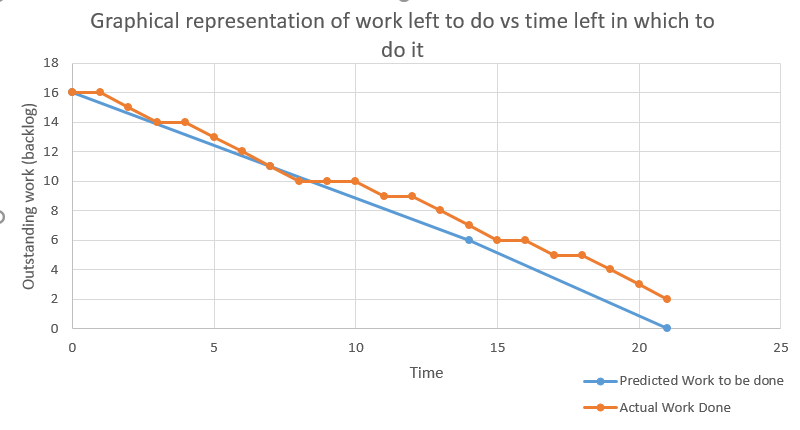
\includegraphics[width=5in]{chart.png}
\caption{Burn chart}
\label{burn down chart of prototype}
\end{figure}

It can be seen from Figure 1.1 that in the beginning of the developmental process of the prototype,the project was on track. However towards the end, the actual work that was being performed was not meeting the targets. This could be because the work that needed to be performed was underestimated and therefore time was not allocated correctly. Care must be taken to ensure that these task are completed in the nearby future, otherwise the project has a high risk of not being completed in time. 

\end{document}